\chapter{Background}\label{chap:background}

This background section will explain some of the concepts, approaches, technologies and software architectures required to understand this thesis.
The findings from the pre-project in \cite{rekstadModelingEnvironmentCloud2020} will also be presented in more detail than the introduction, as the findings are central to this thesis.
Lastly, a section on open source software project management follows, as they shape many of the choices made in the implementation of a solution.

\section{Conceptual Modeling and Model-Driven Development}\label{sec:conceptual-modeling}

\paragraph{Rationale}
\Acrfull{MDD} is the approach to software development which this thesis aims to support.
Therefore, and understanding of \acrshort{MDD} is beneficial, in order to see how an editor should work.

\paragraph{Modeling and abstraction}
The core of \acrshort{MDD} is the model.
The model is a human created construct, formed through humans working together to discuss and refine a problem domain until they reach a consensus of what abstractions help them solve the relevant problems~\cite[p.~154]{brambillaModeldrivenSoftwareEngineering2012}.
Humans perceive the world (and problem domain) as many different phenomena, and conceptual modeling is the act of trying to describe these at some level of abstraction~\cite[p.~1,408]{krogstieModelbasedDevelopmentEvolution2012}.
The model is assumed to resemble the phenomena and work the same way, and yet be simpler than the real world~\cite[p.~414]{krogstieModelbasedDevelopmentEvolution2012}.
Abstraction means to find something common in different observations of a phenomena, and \textit{generalize} their features, \textit{classify} coherent clusters of objects and \textit{aggregate} concepts into more complex ones~\cite[p.~1]{brambillaModeldrivenSoftwareEngineering2012}.
The model will never describe every aspect of the world perfectly, but can \textit{reduce} the world down to relevant aspects, and easily \textit{map} between model elements and real world phenomena~\cite[p.~1-2]{brambillaModeldrivenSoftwareEngineering2012}.


\paragraph{Modeling languages}
In order to describe the model, a \textit{language} is used.
To realize the benefits of \acrshort{MDD}, a \textit{formal language} is used.
The language can be textual or graphical, or both, and imposes a formally defined syntax on the modeler~\cite[p.~13]{brambillaModeldrivenSoftwareEngineering2012}.

\paragraph{Modeling tools}
The advantage of using a formal language is that it can be parsed and understood by software tools, as well as humans.
The tools can validate the model according to the syntax, and to specific rules for the domain.
Tools can also generate code, or execute the model itself.
The model can be transformed into other models, or text or graphics~\cite[p.~8]{brambillaModeldrivenSoftwareEngineering2012}.

\paragraph{\acrlong{MDD}}
The central idea of \acrlong{MDD} is that the model is the source of truth that \textit{drives} the rest of the engineering and development~\cite[p.~9]{brambillaModeldrivenSoftwareEngineering2012}.
There is not a separate model for analysis and for design, but a single one for both~\cite[p.~49]{evansDomaindrivenDesignTackling2004}.
The software code becomes an expression of the model itself, and changes to the code often happen as the result of changes to the model~\cite[p.~49]{evansDomaindrivenDesignTackling2004}.
Because the model and the software are so directly related, the \acrshort{MDD} approach is heavily reliant on tools to automate the tasks of validation and code generation.
The formal language may also sacrifice some of its human readability in order to be understood by tools~\cite[p.~232]{krogstieModelbasedDevelopmentEvolution2012}.
To solve this, one can use other tools that interpret, transform or present models in other ways~\cite[p.~233]{krogstieModelbasedDevelopmentEvolution2012}.
This increases the reliance on tools for \acrshort{MDD} even more, including visual editors.




\section{Model-Driven Development at NTNU in the Course TDT4250}\label{sec:tdt4250}
% * TDT4250. Modeling, use of instances to validate model as you develop, validation of models.

\paragraph{Rationale}
Because the target audience of the software solution (tree editor) are students at \acrshort{NTNU}, it is helpful to know how they work with \acrlong{MDD}.
Their use cases are the ones being solved, meaning the solution must be made with this context in mind.

\paragraph{\Acrshort{MDD} at \acrshort{NTNU}}
To do \acrlong{MDD} effectively, tools should be used.
In the course ``\textit{\gls{TDT4250} Advanced Software Design}''\footnote{Course description is available at \href{https://www.ntnu.edu/studies/courses/TDT4250\#tab=omEmnet}{https://www.ntnu.edu/studies/courses/TDT4250\#tab=omEmnet}.} at \acrshort{NTNU}, the chosen tools are in the \acrfull{EMF}~\cite{hallvardtraettebergEMFTDT4250NTNU2017}.
This includes the modeling language \gls{Ecore}, visual editors in \gls{Eclipse}, model validation logic, the code generator named ``GenModel''\footnote{The code generator is actually named ``codegen'', but users only see the configuration model called ``GenModel''.} (generator model), and more.
\Acrshort{EMF} is a battle-tested technology also used in certain industries, and is well integrated with the \gls{Eclipse}.
The course \gls{TDT4250} also uses \gls{Eclipse} as a case study for other software design concepts, such as modularity (plugin architecture) and dynamic systems (OSGi), and custom \acrlongpl{DSL} which automatically work with \gls{Eclipse}.
\Acrshort{EMF} is relevant for most or all of those concepts.

\paragraph{Development methodology}\label{par:tdt4250-methodology}
Students are taught a methodology or approach for how to do modeling.
They start by specifying a problem space, for example bookkeeping an organization of employees or the courses in \acrshort{NTNU}, and then abstract the problem into a model.
The initial model is externalized as \gls{Ecore} by using a tree editor in \gls{Eclipse}.


Then an \textit{model instance} is made, based on the model, and filled with example data from the domain.
This model instance is used to test and verify that the model is appropriate for the problem space.
Adjustments are made to the model to accommodate any problems with the model instance.


Then validations can be created for the model, by one or both of the following approaches: writing \acrfull{OCL} into model annotations, or marking the model element with an annotation and implementing it as java code.
\Acrshort{OCL} is a \acrlong{DSL} for navigating models and evaluating expressions, and the \gls{Eclipse} can detect annotations with \acrshort{OCL} and evaluate them against the \gls{Ecore} model.
The other option, writing java code, requires the student to first create a new \textit{genmodel} file from the model (by using a menu in \gls{Eclipse}), generating a java code project from the model, and then writing validation logic into the generated code.
For the java code to be picked up, \gls{Eclipse} can start a new instance which installs the generated code as a plugin~\cite{hallvardtraettebergConstraintsValidationTDT42502020}.


Next up, when the model is deemed sufficient, and the most important validations are in place, the student can try to create a user interface.
One of several choices here is to create an \textit{\gls{Eclipse} plugin}.
\Acrshort{EMF} provides code generation for utilities used to integrate the model into an editor for \gls{Eclipse}.
The student uses the genmodel to create these, and tweaks the code if wanted.
Then everything is installed into \gls{Eclipse} by launching a new \gls{Eclipse} instance with the code installed as a plugin.


Lastly, the user interface can be tested.
The student creates a new model instance file, enters some example data from the domain, and runs validation logic.

\paragraph{Lecture materials}\label{par:tdt4250-confluence}
The steps mentioned in the methodology above are available online in \cite{hallvardtraettebergEMFStepbystepTDT42502017,hallvardtraettebergConstraintsValidationTDT42502020,hallvardtraettebergEditingEcoreModel2017,hallvardtraettebergGenmodelTDT4250NTNU2017}.
This is an advantage, because they can by used used in this master's thesis as a basis for creating evaluations and acceptance criteria.



\section{Eclipse Modeling Framework Editors for Ecore}\label{sec:emf-editors}

\paragraph{Rationale}
These editors are the ones being re-implemented in \gls{cloud}-based \acrshortpl{IDE}.
Understanding their functionality and workings is important, as these editors shape the work of this thesis.
The functionalities provided are assumed highly usable and good, because they are the result of many years of work and experience.
This allows this thesis to skip the work of doing usability testing with regards to feature design, as long as the features are similar enough to the copied ones.

\paragraph{Multiple editors}
When editing \gls{Ecore} models in \gls{Eclipse}, there are different editors to pick from.
Usually, \gls{Ecore} models and model instances are saved as \acrfull{XMI}, which is a standardized serialization format based on XML.
The \gls{Ecore} models have the file extension \texttt{.ecore} while model instances either have \texttt{.xmi} or a custom extension for the model, specified by the modeler (e.g. \texttt{.organization} or \texttt{.courses}).
The GenModel has \texttt{.genmodel} as file extension.
However, \gls{Ecore} models are rarely (if ever) edited as XML.
Instead, the files are loaded and presented in a tree structure editor or diagram editor.
These editors are specialized for \gls{Ecore}, and can understand the model.


The diagram based editors use a notation that is based on \gls{UML} Class Diagrams, with boxes, labels and arrows.
Which editor to use can often be a personal preference.
They are all functionally equivalent, with regards to modeling.
The next subsections will describe the most common tree editors in more detail.

\subsection{Sample Reflective Ecore Model Editor}\label{sec:sample-reflective-editor}

The ``\textit{Sample Reflective Ecore Model Editor}'' is one of the main \gls{Ecore} editors in \gls{Eclipse}.
A screenshot of the editor is shown in \cref{fig:sample-reflective-ecore-model}.
The model instances can be edited in a \textit{reflective} editor (without the user first generating java code and installing an \gls{Eclipse} plugin).
Here, reflective means that the editor uses a metamodel (see \cref{sec:emf-metamodel}) for the model instance, and tries to infer the tree structure from containment relationships.


This editor can open both \gls{Ecore} models and model instances.
A screenshot of a model opened in the editor is shown in \cref{sfig:sample-reflective-ecore-model-screenshot}, and a model instance in \cref{sfig:sample-reflective-ecore-model-instance-screenshot}.


This editor is \gls{open source}%
\footnote{Sample Reflective editor source: \href{https://git.eclipse.org/c/emf/org.eclipse.emf.git/tree/plugins/org.eclipse.emf.ecore.editor}{\nolinkurl{https://git.eclipse.org/c/emf/org.eclipse.emf.git/tree/plugins/org.eclipse.emf.ecore.editor}}.}%
, and the editor is itself originally generated by a genmodel~\cite[p.~10]{rekstadModelingEnvironmentCloud2020}.


This editor internally uses a java class called \texttt{ReflectiveItemProvider}%
\footnote{\texttt{ReflectiveItemProvider} source code: \href{https://git.eclipse.org/c/emf/org.eclipse.emf.git/tree/plugins/org.eclipse.emf.edit/src/org/eclipse/emf/edit/provider/ReflectiveItemProvider.java}{\nolinkurl{https://git.eclipse.org/c/emf/org.eclipse.emf.git/tree/plugins/org.eclipse.emf.edit/src/org/eclipse/emf/edit/provider/ReflectiveItemProvider.java}}}
from the \texttt{org.eclipse.emf.edit} \acrshort{EMF} package, to extract text labels and infer icons for the tree view~\cite[p.~10]{rekstadModelingEnvironmentCloud2020}.


For \gls{Ecore} models (with \texttt{.ecore} file extension, not model instances), it uses an \texttt{EcoreItemProviderAdapterFactory}%
\footnote{\texttt{EcoreItemProviderAdapterFactory} source code: \href{https://git.eclipse.org/c/emf/org.eclipse.emf.git/tree/plugins/org.eclipse.emf.ecore.edit/src/org/eclipse/emf/ecore/provider/EcoreItemProviderAdapterFactory.java}{\nolinkurl{https://git.eclipse.org/c/emf/org.eclipse.emf.git/tree/plugins/org.eclipse.emf.ecore.edit/src/org/eclipse/emf/ecore/provider/EcoreItemProviderAdapterFactory.java}}}
to get labels and icons~\cite{edmerksEcoreEditorJava2021}.


These ``item providers'' are especially interesting, because they could be reused in a new editor.

\begin{figure}
    \centering
    \begin{subfigure}[b]{.45\textwidth}
        \centering
        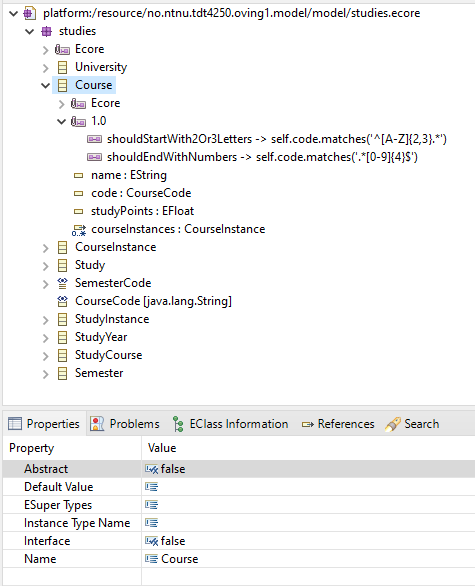
\includegraphics[width=\textwidth]{figures/pre-project/ecore-sample-reflective-ecore-model-editor}
        \caption{A model opened in the editor.}\label{sfig:sample-reflective-ecore-model-screenshot}
    \end{subfigure}
    \hfill
    \begin{subfigure}[b]{.45\textwidth}
        \centering
        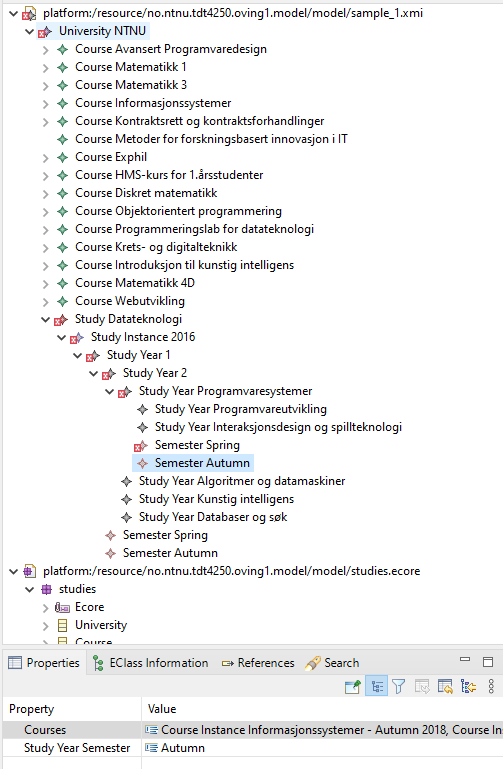
\includegraphics[width=\textwidth]{figures/pre-project/ecore-sample-reflective-ecore-model-editor-instance.png}
        \caption{A \emph{dynamic instance} (\acrshort{XMI} file) opened in the editor.}\label{sfig:sample-reflective-ecore-model-instance-screenshot}
    \end{subfigure}
    \caption{Screenshots of the Sample Reflective Ecore Model Editor in \gls{Eclipse}.}\label{fig:sample-reflective-ecore-model}
\end{figure}


\subsection{EMF Forms Ecore Editor}\label{sec:emfforms-editor}

The \textit{EMF Forms Ecore Editor} is a newer editor than the Sample Reflective editor, and uses EMF Forms\footnote{More info about EMF Forms here: \href{https://www.eclipse.org/ecp/emfforms/index.html}{\nolinkurl{https://www.eclipse.org/ecp/emfforms/index.html}}.} as the technology to provide a user interface~\cite{eclipsesourceEMFFormsEditors2016}.
This editor is \gls{open source}%
\footnote{\textit{EMF Forms} source code: \href{https://git.eclipse.org/c/emfclient/org.eclipse.emf.ecp.core.git/tree/bundles/org.eclipse.emfforms.editor.ecore}{\nolinkurl{https://git.eclipse.org/c/emfclient/org.eclipse.emf.ecp.core.git/tree/bundles/org.eclipse.emfforms.editor.ecore}}.}.
A screenshot of the editor is shown in \cref{fig:emf-forms-ecore-editor}.


This editor is implemented as a generic editor for all \gls{Ecore} model instances, and two subclasses that are specialized for \gls{Ecore} and GenModel~\cite{eclipsesourceEMFFormsEditors2016}.
The generic editor is called \textit{Generic XMI Editor} in \gls{Eclipse}, and the \gls{Ecore} specific editor is called \textit{Ecore Editor}.


The biggest difference compared to the Sample Reflective editor, is how the user interface looks, and that the property sheet is customized based on a \textit{view model file}.
The Sample Reflective editor uses \gls{Eclipse}'s built in property panel.
In the EMF Forms editor, the properties are also grouped into \textit{standard} and \textit{advanced}.

\begin{figure}[htbp]  % order of priority: h here, t top, b bottom, p page
  \centering
  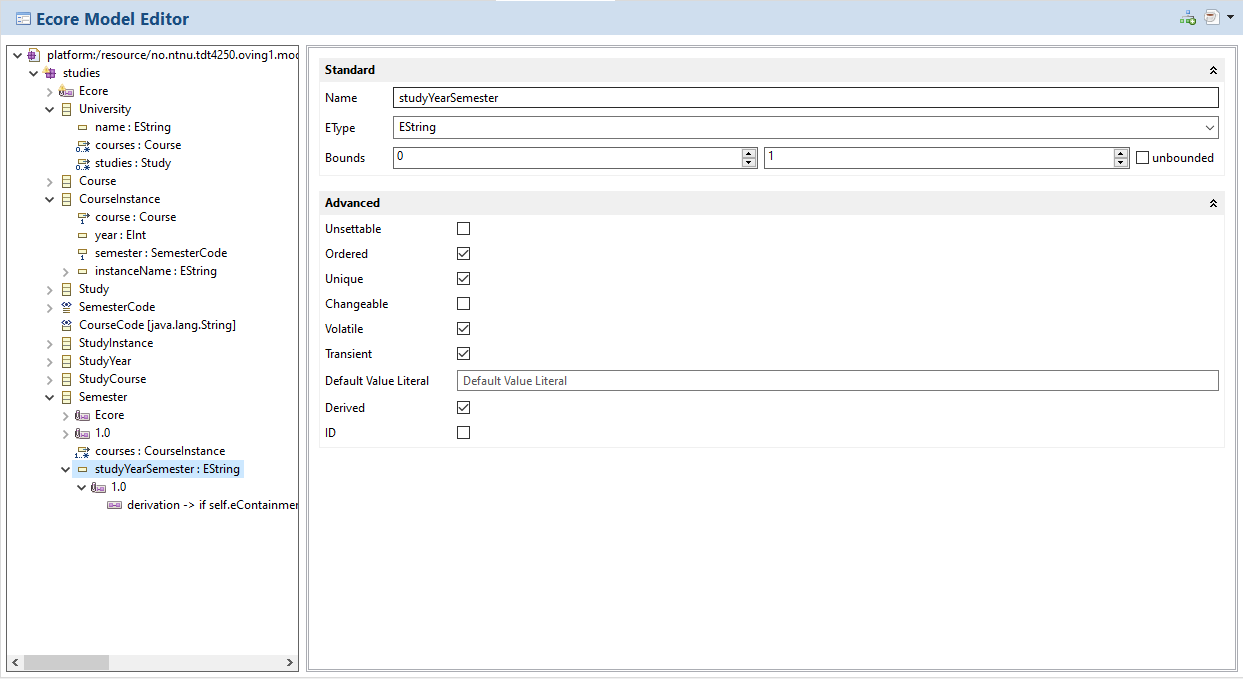
\includegraphics[width=\textwidth]{figures/pre-project/ecore-eclipse-emf-forms-model-editor.png}
  \caption[EMF Forms Ecore Editor]{A screenshot of a model in the EMF Forms based Ecore Editor.}\label{fig:emf-forms-ecore-editor}
\end{figure}

\iffalse{} 
{
%Skip diagrams for now. Tree editors are more important.

  \subsection{Ecore Tools diagrammatical editor}\label{sec:ecore-tools-editor}
  
  The \textit{Ecore Tools} editor presents \gls{Ecore} as class diagrams, similar to \gls{UML} Class Diagrams.
  
  \subsection{EMF.Cloud ecore-glsp diagrammatical editor}\label{sec:ecore-glsp-editor}
  %TODO
  
}
\fi


%* Eclipse EMF offers different Ecore editors. Tree-editor is important for developers, and diagrams are important in runtime and end-users.



\section{Introduction to Tree Structures}\label{sec:tree-structures}

\paragraph{Rationale}
Because the editors center around a tree structure, a clear understanding of trees is helpful.

\paragraph{Trees}
A \textit{tree} is a data structure.
The tree is composed of \textit{nodes}, and one node is designated as the \textit{root node} node or \textit{tree root}.
Each node can have zero or more \textit{children} nodes, and one \textit{parent} node.
The root node does not have a parent.
When representing the tree as code, it is possible to omit either the parent or child relationship in a node, making the parent or child implicit.
The relationship can still be found, by \textit{traversing} the tree.
Traversing means to visit every node it the tree by following the parent or child relationships.


\paragraph{Visualizing trees}
There are many ways to present trees to humans.
Two common approaches are \textit{hierarchy} and \textit{diagram}.


In a hierarchy, the parent is presented as a row, and its children on separate rows below (see \cref{sfig:tree-visualized-hierarchy}).
The children are often indented as well, and possibly connected with dots or lines to the parent.


In a diagram, nodes are often displayed as a circle or box (see \cref{sfig:tree-visualized-diagram}).
The parent is displayed above its children, and the children are aligned on the same row.
The parent-child relationship is shown as a line or arrow, connecting the parent to the child.

\begin{figure}[htbp]
    \centering
    \begin{subfigure}[b]{.45\textwidth}
        \centering
        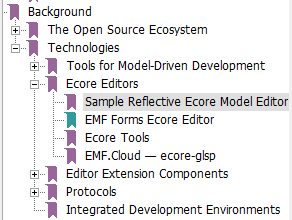
\includegraphics[width=\textwidth]{figures/tree-hierarchy.png}
        \caption{A tree visualized as a hierarchy. The top node is the root.}\label{sfig:tree-visualized-hierarchy}
    \end{subfigure}
    \hfill
    \begin{subfigure}[b]{.45\textwidth}
        \centering
        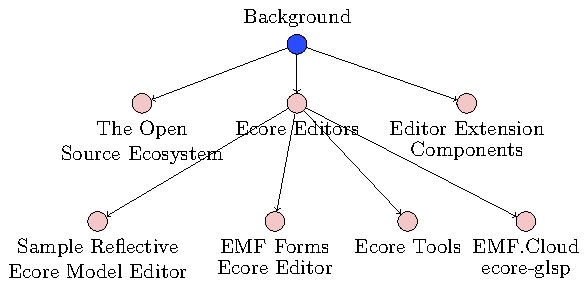
\includegraphics[width=\textwidth]{figures/tree-diagram.pdf}
        \caption{A tree visualized as a diagram. The blue node at the top is the root.}\label{sfig:tree-visualized-diagram}
    \end{subfigure}
    \caption{A tree visualized as a hierarchy and diagram. The labels are section titles of \cite{rekstadModelingEnvironmentCloud2020}, as an example.}\label{fig:tree-visualized}
\end{figure}

\paragraph{Nodes}
The tree is more useful when the nodes have properties.
The minimum property is children or parent.
But a useful property is a name, label or id, with regards to presenting the tree to a human.
There may be properties on the relationships between a node and its children, but these may be hard to present visually in hierarchy-type visualizations.
For a diagram type visualization, the properties may be presented as labels on the edge.

\paragraph{Mapping to trees}
A data structure can be mapped to a tree if it has separate objects with a containment or aggregation relationship.
There can be different ways to map to a tree, depending on what properties are used (or not used).
The labels can also come from various object properties, be derived from them or combine multiple properties into one label.



\section{Master-Detail Tree Editor}\label{sec:master-detail}

\paragraph{Rationale}
The tree editors use a layout pattern called \textit{master-detail}.

\paragraph{Description}
As the name \textit{Tree Editor} implies, they are used to edit a tree.
There are mainly two different things that can be edited: the parent-child relationships and the node's properties.
The user interfaces for the tree editors in \cref{sec:emf-editors} use a pattern called \textit{master-detail}.
This means the user interface is composed of two parts: a \textit{master view} and a \textit{detail view}.
% TODO: add a figure of master-detail overlayed on an editor?


\paragraph{Master view}
The tree structure is shown as a hierarchy in the master view.
It is common for the master view to be positioned to the left of a detail view, or above it.
The user interacts with the master view to add, remove and select nodes.
Adding a new child to a parent is done here.


\paragraph{Detail view}
When a node is selected, its properties are displayed in the detail view.
It is common for the detail view to be positioned to the right of a master view, or below it.
The detail view is usually a \textit{input form} or tabular (rows and cells) structure.
The user usually enters text, numbers, ticks checkboxes and opens selection dialogues from the detail view.


\section{The Eclipse Reflective Ecore Editor}

* Reflective Ecore Editor, its architecture, Commands in .Edit, works on any model.
* Adaptation of editors to special cases like Ecore model and Genmodel.
% TODO: remove? DUplicate of prev. section?

\section{An Overview of EMF:\ Ecore Metamodel, XMI Serialization and GenModel for Code Generation}\label{sec:emf-metamodel}


\paragraph{Rationale}
The \acrfull{EMF} is the \acrlong{MDD} framework used in \gls{TDT4250}.
The tree editor will modify \gls{Ecore} models, so it helps to understand the concepts and names used in the \gls{Ecore} metamodel.
It is also useful to know the different tools and components in \acrshort{EMF}, because the tree editor intends to reuse as much of them as possible internally, to save development effort.

\paragraph{\acrlong{EMF}}
The \acrfull{EMF} is a part of the Eclipse Modeling project from the Eclipse Foundation.
It is a framework and code generation facility that lets developers define models.
The models can be java code, \gls{XMI} or \gls{UML}, and the other two can be generated~\cite[p.~14]{edmerksEMFEclipseModeling2009}.
This framework may be chosen as the tools for doing \acrlong{MDD} (see \cref{sec:conceptual-modeling}).
In EMF, the models are expressed with the \gls{Ecore} modeling language.
This modeling language is similar to \gls{UML} Class Diagrams, in terms of the concepts and what it can express~\cite[p.~16]{edmerksEMFEclipseModeling2009}.
The real world data that could fit inside a specific model is called a \textit{model instance}.

The framework was made to take use of the editing capabilities and utility of the \gls{Eclipse}~\cite{edmerksEMFEclipseModeling2009}.
This means that there is much tooling and integration for \acrshort{EMF} with \gls{Eclipse}.
For example, EMF can generate a plugin to edit model instances in \gls{Eclipse}.

%TODO
% eclipse editor plugins, language, codegen, ocl, serialization format

\paragraph{\Gls{Ecore} metamodel}
The modeling language in \acrshort{EMF} is \gls{Ecore}.
A \textit{metamodel} is the model of a model.
This means that Ecore is the metamodel for all models expressed using \acrshort{Ecore}.
Ecore is itself modeled in Ecore, so it is its own metamodel.


\paragraph{Model concepts}
The main concepts used in \gls{Ecore} to model, are \texttt{EClass}, \texttt{EAttribute}, \texttt{EReference} and \texttt{EDataType}%
\footnote{The name Ecore comes from EMF Core, and the `E' prefix for \texttt{EClass} etc.\ come from Ecore.}.
These are distinct objects with names, properties and inheritance, like in object oriented programming.
As for the metamodel, \texttt{EClass}, \texttt{EAttribute} and \texttt{EReference} are all extending \texttt{ENamedElement}, which defines their \texttt{name} property~\cite{edmerksEMFEclipseModeling2009}.

When modeling, \texttt{EClass} is used to create java classes.
The \texttt{EAttribute} and \texttt{EReference} are used to model class properties, like member variables.
An \texttt{EAttribute} defines a property, such as e.g. \textit{age} or \textit{address}, while \texttt{EReference} defines a reference/association to another \texttt{EClass}, e.g. \textit{parent} or \textit{order}.
The \texttt{EAttribute} has a attribute type, the \texttt{EDataType}, which can be e.g. \texttt{EInt} or \texttt{EString}~\cite{edmerksEMFEclipseModeling2009}.

Java class methods are modeled with another concept, the \texttt{EOperation}.
Lastly, everything in the model lives inside an \texttt{EPackage}, which represents a java package (or other kind of code module).
There are more concepts in \gls{Ecore}, but many are only used internally as part of the metamodel, to represent \gls{Ecore} itself.


\paragraph{\Acrshort{XMI} serialization}
When an \gls{Ecore} model is written as a text file, it needs \textit{serialization}.
The official format for serializing Ecore is \acrfull{XMI}.
This format is based on \acrfull{XML}.
The file extension is usually \texttt{.ecore}.
Model instances can also be serialized as \acrshort{XMI}, and have custom file extensions or \texttt{.xmi}.
It is also possible to serialize \gls{Ecore} to other formats, like \gls{JSON}, using third party tools.
% serialization, standardized EMOF, default for ecore, XML,

\paragraph{\acrshort{EMF} runtime java \acrshort{API}}
The java code generated by \acrshort{EMF} will by default extend a set of java classes defined by \acrshort{EMF}.
Instead of a generated \texttt{EClass} extending \texttt{java.lang.Object}, it extends \texttt{EObject}.
And instead of using an \texttt{ArrayList}, a collection in \gls{Ecore} will use a \texttt{EList}.
When creating a new instance, the class constructor is not used, but a Factory instance on the generated \texttt{EPackage} for the model.


All of these framework java-classes are the \acrshort{EMF} java \gls{API}.
They provide much of the power, flexibility, reflection and meta-modeling capabilities of \acrshort{EMF} in java.
For example, a program can work with a \acrshort{EMF} model without knowing the code beforehand, by using the reflection \acrshort{API} to retrieve names and properties of a model object.


The \acrshort{API} also provides utilities for working with the model.
There are \acrshortpl{API} for listing the children of an \texttt{EObject}, getting a human representation of it, and for modifying and observing state changes.
Another important \acrshort{API} is the \texttt{ResourceSet} and \texttt{Resource}, used to read and save models to serialized \acrshort{XMI} files.

\paragraph{GenModel code generation}
Code generation is an important part of \acrshort{EMF}.
The generator can be configured with its own generator model, nicknamed the \textit{GenModel}.
This model holds options for how the code will be named, what templates should write the code, if the code can use the \acrshort{EMF} \acrshortpl{API}, and more.
This model is itself an \gls{Ecore} model, and has an \texttt{.genmodel} file extension~\cite[p.~28]{edmerksEMFEclipseModeling2009}.


The generator can also produce more than just a java representation of the model.
A test suite can be generated, with an empty test skeleton for the generated code.
It can also generate utilities for creating model editors, in what is called the \textit{.edit} java package.
The name ``.edit'' is appended to the original package name.
This has \textit{ItemProvider} classes which helps an editor to find the human representations, properties, child objects, and to notify on changes.


Another utility is related to the \gls{Eclipse}, which is the \textit{.editor} java package.
This holds key classes for integrating with \gls{Eclipse}, making it a custom editor.
For example, custom actions, project wizards, eclipse plugin logic is part of this.


\paragraph{Custom code}
The generated code must usually be modified by a developer.
This can be to fill in the implementation of a \texttt{EOperation}, or tweak some behavior.
The generated code has a \texttt{@Generated} java annotation, which the developer changes to prevent the code generator from overwriting the method body.


\section{Visual Studio Code and Theia}

The two \acrshortpl{IDE} relevant for this thesis are Visual Studio Code (\gls{VSCode}) and \gls{Theia}.
Both are available as editors in \gls{Gitpod} as cloud based \acrshortpl{IDE}.

\subsection{Visual Studio Code}

\Gls{VSCode} is a very popular \gls{open source} \acrshort{IDE} created by Microsoft~\cite{stackoverflowStackOverflowDeveloper2019}.
A screenshot is shown in \cref{fig:vscode-ui}.
It uses web technologies like javascript, \gls{Nodejs} and \gls{Electron} to provide an advanced text editor and tools for programming on a desktop.
Originally made only for desktop, \gls{VSCode} was later adapted to also work in a browser when \gls{GitHub}\footnote{GitHub is owned by Microsoft.} launched Codespaces~\cite{svenefftingeProductRoadmapQ1}.
\Gls{VSCode} is extensible, and allows third party developers to create extensions.
These are distributed from Microsoft's extension store: Visual Studio Marketplace\footnote{Marketplace website: \href{https://marketplace.visualstudio.com/vscode}{\nolinkurl{https://marketplace.visualstudio.com/vscode}}.}.

\paragraph{Programming languages}
One common use of extensions is to support new programming languages.
The text editor in \gls{VSCode} is a generic text editor component called \textit{Monaco}~\cite{benjaminpaseroSourceCodeOrganization2020}.
This same text editor is used for all programming languages.
For the text editor to know the keywords, suggestions and other specifics of a programming language, the extension uses a standardized protocol to inform Monaco.
This protocol is called the \acrlong{LSP}, and is described in \cref{sec:lsp}.

\begin{figure}[htbp]  % order of priority: h here, t top, b bottom, p page
  \centering
  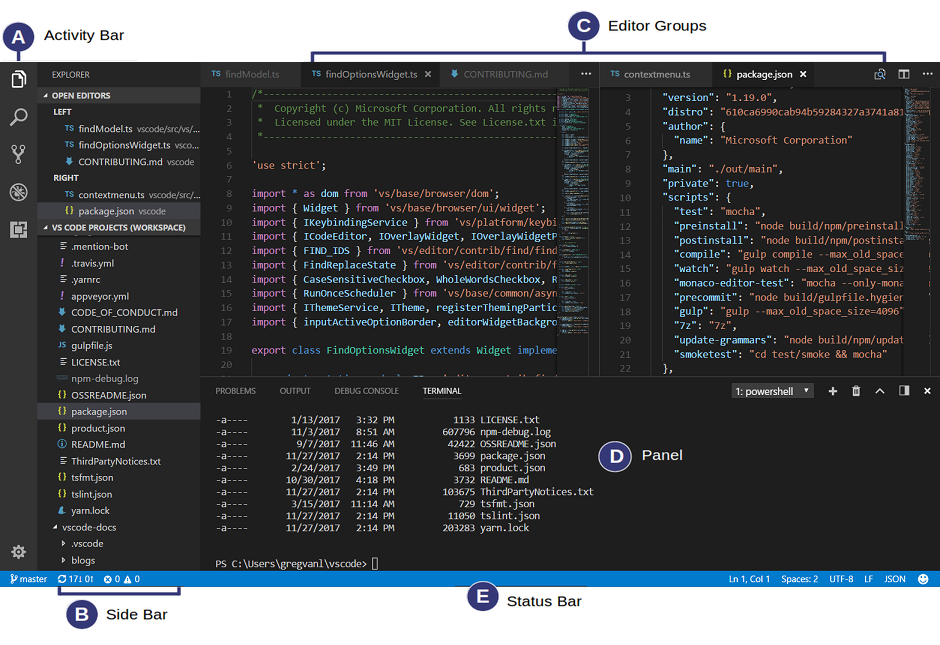
\includegraphics[width=\textwidth]{figures/pre-project/vscode-ui.png}
  \caption[VSCode User Interface]{The \gls{VSCode} user interface, annotation with the different components (A-E).}\label{fig:vscode-ui}
\end{figure}

\subsection{Theia}

Theia is based on the \gls{open source} components from \gls{VSCode}, without a proprietary component that Microsoft added for telemetry.
Theia is managed by the Eclipse Foundation, and was created to be web based from the start (before Codespaces launched, when \gls{VSCode} was desktop only).
A screenshot is shown in \cref{fig:theia-ui}.
The main uses of Theia are workspace services like \gls{Gitpod} and Eclipse Che, but it is also intended to be a ``web based version'' of the Eclipse Rich Client Platform.
This means tools can create their own distribution of Theia, where they are deeply integrated~\cite{helmingEclipseTheiaIDE2019a}.

\begin{figure}[htbp]  % order of priority: h here, t top, b bottom, p page
  \centering
  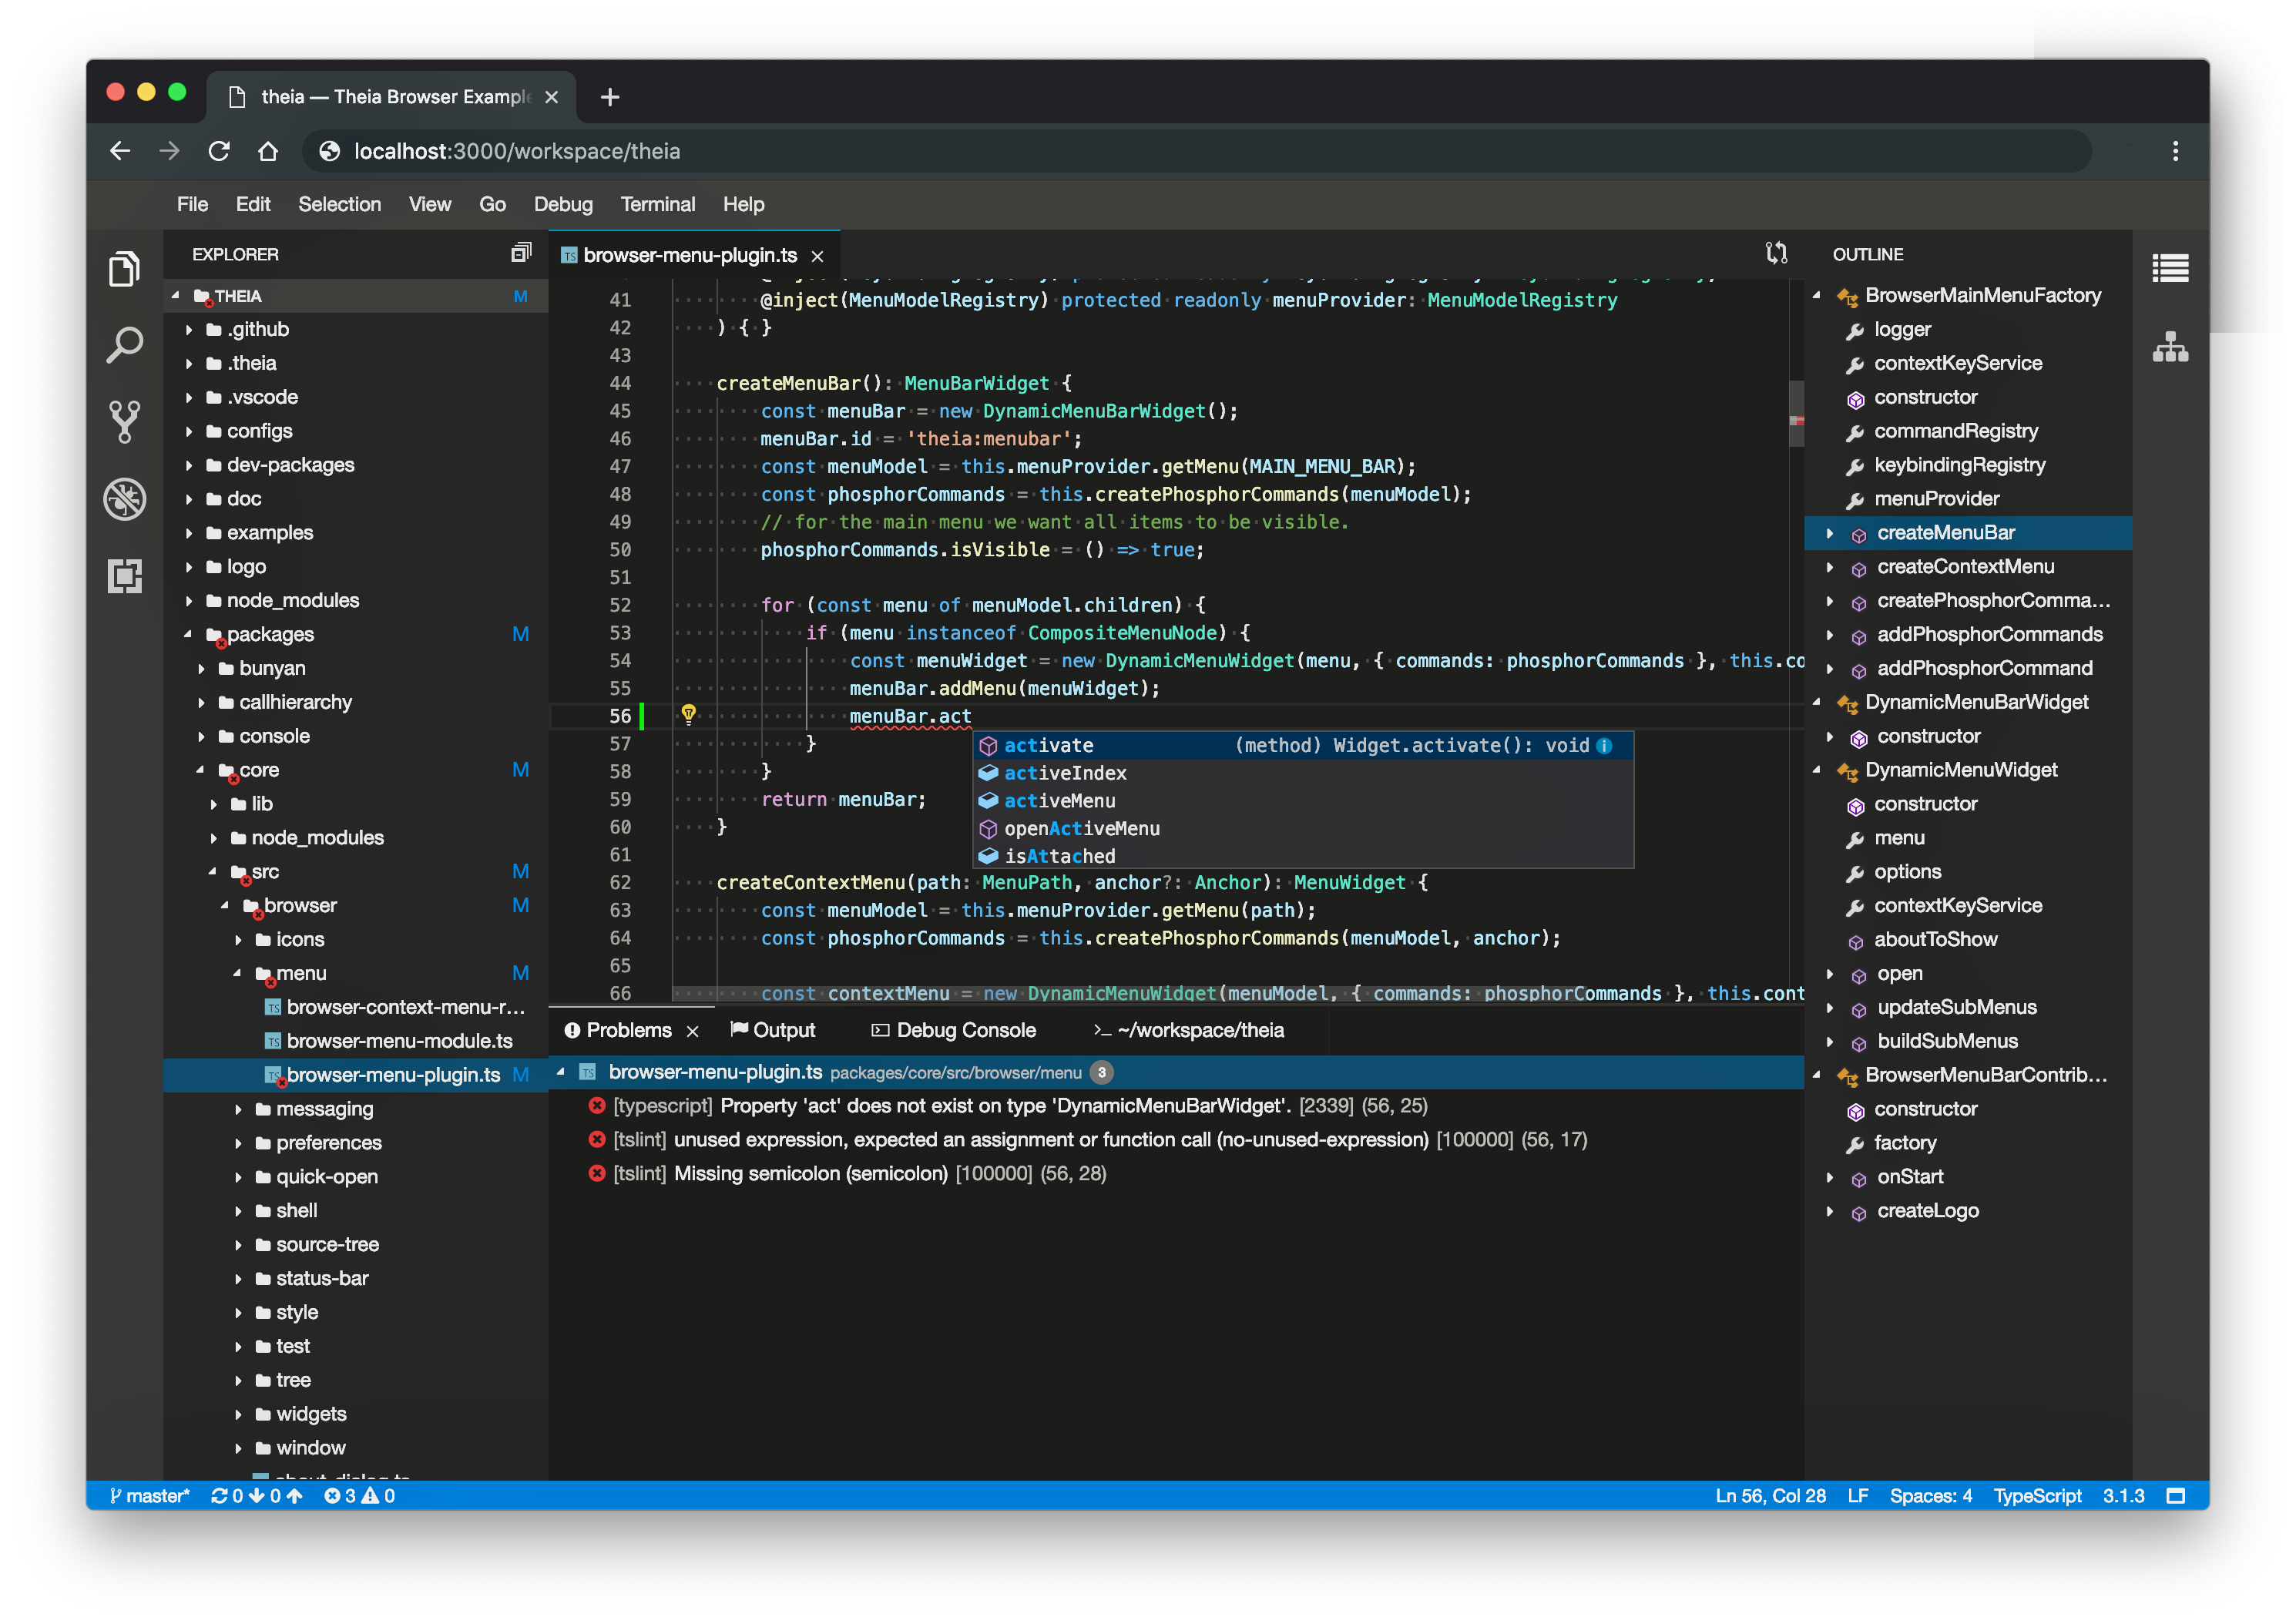
\includegraphics[width=\textwidth]{figures/pre-project/theia-screenshot.png}
  \caption[Theia User Interface]{The \gls{Theia} user interface.}\label{fig:theia-ui}
\end{figure}

\paragraph{Extensions}
Theia can load extensions using the same \acrfull{API} as \gls{VSCode}.
Theia calls these ``Theia Plugins''.
Another way to extend Theia is using ``Theia Extensions''.
These have full control over the \acrshortpl{IDE}, and can modify practically anything.
Installing a Theia Extension requires the user to perform a full compilation of \gls{Theia} itself~\cite{helmingHowAddExtensions2019}.
A Theia Plugin (or \gls{VSCode} extension) however, can be installed at runtime.
Because of licensing issues with Microsoft and the Visual Studio Marketplace, Theia Plugins are instead hosted at a independent marketplace called \textit{OpenVSX}~\cite{svenefftingeOpenVSX2020}.


\section{Visual Studio Code's Custom Editor API}\label{sec:vscode-custom-editor}

A \gls{VSCode} extension is allowed to use a set of \acrlongpl{API} provided by \gls{VSCode}.
One such \acrshort{API} is the \textit{Custom Editor API}.
This allows an extension developer to create \textbf{custom editors other than text editors}.
This could be diagrams, pictures, graphs, or \textbf{trees}, for example.
The developer has the full freedom of a web browser, as they are given their own isolated frame.
Normally, an extension cannot modify the user interface outside of the provided \acrshortpl{API}.
This is in contrast to inside the provided \texttt{WebView}, where the developer has to \textit{create and manage} the entire user interface.
In addition to a user facing \texttt{WebView}, the developer must create their own document model.
By default, \gls{VSCode} uses a document model for text documents, with selections, edits, versions and more.
The \texttt{CustomDocument} only has a uri pointing to the file.
Another central part is the \texttt{CustomEditorProvider}, with a few methods to fill in, like opening, undoing and saving a document.




\section{Language Server Protocol Architecture}\label{sec:lsp}
%TODO
* LSP from VSCode solves language-to-editor m*n combinations. There is already a need to move EMF from Eclipse to VSCode, it might need to move to IntelliJ etc. in the future.
* Monaco general frontend. Also Eclipse uses LSP with JDT? IntelliJ??
* Base protocol \label{sec:base-protocol}

\section{JSON-RPC}
%TODO

\section{\Gls{cloud} and \gls{Gitpod}}

\paragraph{Cloud}
The \gls{cloud} is the term used for rented computing power and data storage in data centers owned by third parties.
This is in contrast to in-house or on-premise servers.
An advantage of running software in the \gls{cloud} is that maintenance of hardware is out sourced.
If a hard drive or processor breaks down, it is the cloud vendor's responsibility to fix, and to provide failover mechanisms so a customer is not impacted.


Another advantage is the ability to scale up or down instantly on demand.
If a on-premise server is overloaded, the organization has to purchase more servers and configure them.
Just the shipping of hardware alone takes more time than requesting more compute power from a \gls{cloud} provider.
The cloud providers usually have so large data centers that they never ``run out'', as long as a customer is able to pay for it.
Some of the best known cloud providers today are Amazon with Amazon Web Services, Google with Google Cloud, and Microsoft with Azure.

\paragraph{Gitpod}
Gitpod is a \gls{cloud} based \acrfull{IDE}.
It is provided as a service, or it can be self hosted.
The idea behind \gls{Gitpod} is that a developer does not need to install the tools on their own machine.
Instead, a machine is provisioned at a cloud provider, and any tools are installed there.
The developer interfaces with this machine through a web based \acrshort{IDE}.
For Gitpod, the default \acrshort{IDE} is \gls{Theia}.
The source code is downloaded from an online source code host, such as \gls{GitHub}, and into a workspace on the provisioned machine. %TODO: cite?



\section{\acrlong{EMF} in the \Gls{cloud}}\label{sec:emf-in-cloud}
%TODO
* Recent development, EMF.Cloud Model Server, EMF.Cloud EMFJson, GLSP, GLSP Ecore Editor (and ActionMessage\label{par:glsp-actionmessage}), GLSP Coffee Editor, JSON Forms.
Theia Tree Editor\label{par:theia-tree-editor} (source: \cref{EclipseemfcloudTheiatreeeditor2020}. Schemas and child mapping at \cref{EclipseemfcloudCoffeeeditor2021}. Tutorial: \cref{helmingHowBuildTree2021}) and coffee-example, for those able to compile Theia.

\section{Pre-project Results}

\subsection{Research Questions}

The pre-project started by asking the following research question:
\begin{quote}
\textit{How can we modernize Model-Driven Development Frameworks to appeal to
the next generation of software developers, using recent developments in cloud
IDEs?}~\cite[p.~3]{rekstadModelingEnvironmentCloud2020}
\end{quote}

After answering this question, the pre-project narrowed down to the following research question:

\begin{quote}
\textit{How can we design an Ecore master-detail tree editor that works in both VSCode and Theia, while reusing existing tools for Ecore such as codegen and validation?}~\cite[p.~24]{rekstadModelingEnvironmentCloud2020}
\end{quote}

A set of five related sub-questions were also posed, and subsequently answered.
These questions set the context for a solution, and the stakeholders, constraints and requirements that would be needed.
The following subsections (\ref{subsec:stakeholders} to \ref{subsec:pre-project-protocol}) will present the results of the pre-project that are the basis of work done in this thesis.

\subsection{Stakeholders}\label{subsec:stakeholders}

A stakeholder is someone affected by or interested in the solution.
It can be an organization or people~\cite[p.~52]{bassSoftwareArchitecturePractice2013}.
The pre-project identified the key stakeholders in \cite[p.~3]{rekstadModelingEnvironmentCloud2020} to be:

%TODO use a table?
\begin{itemize}
  \item Kristian Rekstad (author). Goal: increase adoption of \acrshort{MDD} by students and industry. Has to design and develop the initial solution.
  \item Hallvard Trætteberg (supervisor). Goal: teach students the concepts of \acrshort{MDD} in \gls{TDT4250}. Wants to use \gls{Gitpod} and \acrshort{EMF} for student assignments.
  \item Teachers/Lecturers that use \acrshort{EMF}. Goal: teach students. Have to present the tree editor, use it and support students that ask for help.
  \item Students. Goal: learn useful technologies and pass courses like \gls{TDT4250} to get a grade. Will have to use \acrshort{EMF} if they study Computer Science with the ``Software Engineering'' specialization at \acrshort{NTNU}.
  \item Industry professional using \acrshort{EMF} to do \acrshort{MDD}. Goal: develop software for a business/client. May want to use \acrshort{EMF} without using \gls{Eclipse}, for personal reasons or organization policy.
  \item Eclipse Foundation. Goal: foster a community of developers and provide open source software. The maintainers of \acrshort{EMF}.
  \item Eclipse ecosystem developers. Goal: contribute to Eclipse Foundation projects. May possibly have to maintain and further develop this (or a derivative) solution if this project succeeds and they embrace it.
  \item Developers of third party \gls{VSCode} extensions that use tree editors. Goal: provide a high quality editor for their specific problem domain. Could use the architecture, protocol and frontends of this solution, if this solution is high enough quality, architected to be reusable and partially independent of \acrshort{EMF}, and reuse will reduce their design and/or development time.
\end{itemize}

\subsection{Software Requirements}

\paragraph{Requirement engineering approach}
The pre-project tried to establish the software requirements for a tree editor.
A literature review failed to find related works that listed the requirements for a tree editor.
The literature review also failed to find related works for modeling in the cloud with the purpose of creating \gls{Ecore} models.
The related works either \textit{deployed} \gls{Ecore} models to the cloud, were textual editors, or did not use \gls{Ecore}~\cite[p.~3]{rekstadModelingEnvironmentCloud2020}.\\

Without literature to suggest requirements, and without users to test on (except the author and supervisor), the best option was to analyze the existing tree editors in \gls{Eclipse}.
Common modeling tasks were performed (see \cref{par:tdt4250-confluence}), and detected functionality was recorded.
The result gave an initial list of functional requirements, but not a complete one.
However, by following an agile approach instead of waterfall, this list does not need to be complete\footnote{Agile values working software over extensive documentation, thus spending time on creating a working solution is better than a ``worthless'' list of everything a solution \textit{could have done}.}.
More requirements will emerge naturally as work progresses.
Still, having a good overview of the requirements is needed to correctly decide a software architecture, because of ``architecturally significant requirements'' that affect the architecture~\cite[p.~291]{bassSoftwareArchitecturePractice2013}.

\paragraph{Constraints}
A constraint is a restriction on the available choices for a solution~\cite[p.~7]{wiegersSoftwareRequirements2013}.
The most important constraint discovered was that the tree editor must be a \gls{VSCode} extension.
There is an alternative extension mechanism for \gls{Theia}, which was deemed incompatible with \gls{Gitpod}%
\footnote{Gitpod can use Theia as its editor frontend, but the user is not allowed to recompile and upload a new version of Theia. The alternative extension mechanism, \textit{Theia Extensions} needs a full recompilation of Theia~\cite[p.~38]{rekstadModelingEnvironmentCloud2020}. However, VSCode extensions can be installed during runtime, also in Theia in Gitpod.}%
~\cite[p.~38]{rekstadModelingEnvironmentCloud2020}.


\paragraph{Functional requirements}
A functional requirement specifies \textit{what} a solution must do, such as supported features~\cite[p.~7]{wiegersSoftwareRequirements2013}.
The pre-project identified several functional requirements for a tree editor in the cloud.
The full list of functional requirements, with id, requirement and description can be found in \cref{app:functional-requirements}.
The list can be summarized as follows:

\begin{itemize}
  \item Provide a master-detail tree editor in VSCode and Theia (Gitpod) by using an extension mechanism of the \gls{IDE}.
  \item The tree editor must show nodes with labels and icons as a hierarchy.
  \item Allow selecting a node in the tree editor by clicking it.
  \item Provide a property sheet for the selected node in the tree editor.
  \item Provide an action bar with actions that can be dynamically specified by a backend server.
  \item Child nodes can be hidden or shown in the tree by a user.
  \item The tree editor and property sheet must update when the underlying model changes in the server.
  \item The action bar shows appropriate actions based on the selected node.
  \item The tree editor must allow creation of new nodes.
  \item The tree editor must allow deleting nodes.
\end{itemize}

Some more important requirements were implicit, and not defined in the list.
This was not intentional, and an evidence to the list's non-completeness.
Some of the implicit requirements are explicitly defined as follows:

\begin{itemize}
  \item The editor must handle \gls{Ecore} models.
  \item The editor must handle model instances from \acrshort{XMI} files.
  \item The tree structure must be based on containment properties in the \gls{Ecore} model.
  \item The editor must provide a command in the \acrshort{IDE} to create a new \gls{Ecore} file with the minimum \acrshort{XMI} needed for a valid empty model.
  \item Tree nodes can be moved to new parents by drag-and-drop by the user.
  \item The drag-and-drop can not let the user drop a node on a parent that cannot contain the node as a child. 
  \item Saving a model will serialize it as \acrshort{XMI} to a file on disk.
  \item An action in the action bar must be added to run \textit{model validation}.
  \item An action in the action bar must be added to run \textit{code generation}.
  \item The editor shall show multiple tree roots when there are related model files. Opening a \gls{Ecore} file shall also show any genmodel file. A model instance shall also include a root for the \gls{Ecore} model in the same editor.
  \item A user can open more than one unique \gls{Ecore} model at the same time, in separate ``tabs'' in the editor.
  \item Any modification to the model must support undo and redo.
\end{itemize}


\paragraph{Non-functional requirements}
A non-functional requirement specifies characteristics or properties of the solution~\cite[p.~7]{wiegersSoftwareRequirements2013}.
Most of the non-functional requirements are grounded in empirical evidence like what the Eclipse ecosystem and web development ecosystems are currently doing.
A non-formal list of the non-functional requirements is as follows:

\begin{itemize}
  \item Compatibility with a code editor in \gls{Gitpod}.
  \item Use a permissive \gls{open source} license.
  \item Avoid software dependencies that are closed-source or use restrictive licenses.
  \item Use a distributed architecture with components reusable in other \acrshortpl{IDE}, inspired by architectures already in use by similar solutions~\cite[p.~24]{rekstadModelingEnvironmentCloud2020}.
  \item Configurability of user-facing options. Choices of colors, fonts, file system paths and similar should be possible to change~\cite[p.~24]{rekstadModelingEnvironmentCloud2020}.
  \item Configurability of mapping of \gls{Ecore} models to trees. Which containment references to use as children, and custom logic for labels should be user-specifiable~\cite[p.~24]{rekstadModelingEnvironmentCloud2020}.
  \item Localize the user interface in English.
  \item Flexibility and extensibility in the protocol to the server, allowing custom messages~\cite[p.~24]{rekstadModelingEnvironmentCloud2020}.
\end{itemize}


\subsection{Architecture and Protocol for a Solution}\label{subsec:pre-project-protocol}

A specific software architecture was proposed.
It had a goal to solve the requirements for: software reuse, \gls{Theia} and \gls{VSCode} compatibility, tree hierarchy editing, and a solution that could be transferable to other tree domains and editors.
Additionally, the protocol would try to stay close to related solutions, as they are empirically tested and familiar to developers in the Eclipse ecosystem.
By creating prototypes, major ``blockers'' or risk factors of the proposed architecture was tested and proven non-problematic~\cite[p.~38-46]{rekstadModelingEnvironmentCloud2020}.


\subsubsection{Architecture}

The tree editor shall be a \gls{VSCode} extension, and use the available \acrlongpl{API} for \gls{VSCode} extensions.
No dependencies to \gls{Theia} shall be introduced.
To view the tree structure as a hierarchy, the \textit{Custom Editor API} in \gls{VSCode} must be used (see \cref{sec:vscode-custom-editor}).
A custom editor can present the editor inside \gls{VSCode} as a \textit{WebView}, meaning a custom webpage free to render anything, isolated from the rest of \gls{VSCode}.


\paragraph{Components}
The editor thus comprises 4 components: the tree editor WebView (``\textbf{editor frontend}''), the \gls{VSCode} extension integration (``\textbf{extension}''), a \textit{Tree Language Server} (``\textbf{TLS}'') and the \textit{EMF.Cloud ModelServer} (``\textbf{ModelServer}'')~\cite[p.~48,49]{rekstadModelingEnvironmentCloud2020}.
An illustration is shown in \cref{fig:pre-project-tree-editor-architecture}

\begin{figure}[htbp]
  \centering
  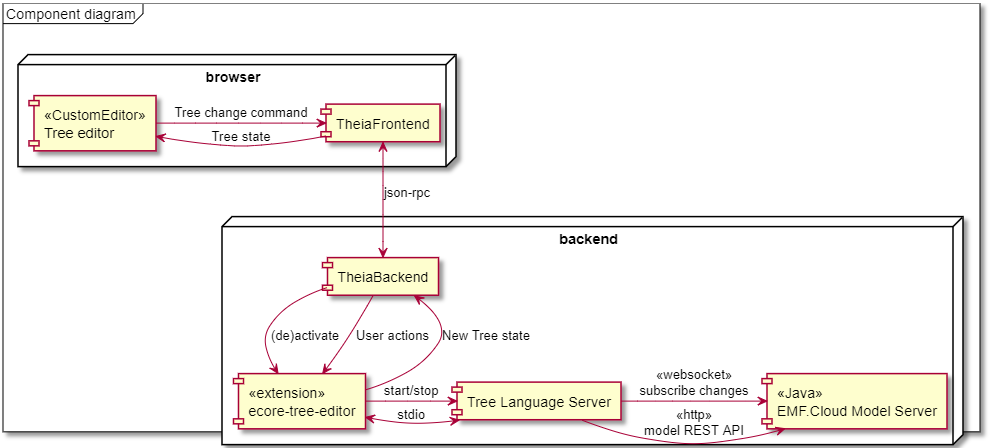
\includegraphics[width=\textwidth]{figures/pre-project/tree-editor-component-diagram.png}
  \caption[Tree Editor Architecture]{A suggested architecture for a tree editor. Copied from Figure 5.15~\cite[p.~49]{rekstadModelingEnvironmentCloud2020}. The diagram is based on \gls{Theia}, and the \gls{JSON-RPC} between TheiaFrontend and TheiaBackend happens behind the scenes, and is therefore not relevant to discuss.}\label{fig:pre-project-tree-editor-architecture}
\end{figure}


\paragraph{Editor frontend}
The editor frontend must be a web application that renders the tree as HTML, and provides interactivity with javascript. 
It communicates to the extension using \textit{messages} containing \gls{JSON}\footnote{This is a constraint imposed by the WebView API in VSCode.}.
The editor frontend will send messages that are \textit{commands} with the changes or actions a user triggered.
The extension will send messages with the new tree state to be shown.

\paragraph{Extension}
The extension is the main artifact which a user will install into \gls{VSCode} or \gls{Theia}.
This must be implemented with the \gls{TypeScript} language or javascript.
The extension will bundle the compiled code for the editor frontend, TLS and ModelServer inside it.
The extension is responsible for integrating with the \gls{IDE}, so that model files are opened in the custom editor, and handles commands triggered by the user in the \gls{IDE} (such as actions to create a new file, or saving a model).
The extension will start and stop the TLS process, and communicate over a \gls{JSON-RPC} protocol or \gls{REST} plus \gls{WebSocket}.
The extension and TLS can either use TCP sockets or standard in/out as the transport.

\paragraph{TLS}
A Tree Language Server (TLS) will contain specific knowledge about \gls{Ecore} and \acrshort{EMF}.
The choice of programming language is unconstrained.
The main purpose of the TLS is informing the extension of tree state, provide configuration for the tree editor and extension, and receive commands to modify models.
The TLS must be able to communicate using the same protocol as the extension (\gls{JSON-RPC} or \gls{REST} and \gls{WebSocket}), and either do so over standard in/out, or listen to incoming TCP sockets.
The TLS will perform commands to modify \acrshort{EMF} models by using as much re-use of existing code and frameworks as possible.
The TLS will start the ModelServer and communicate with it to read and modify models.
The ModelServer is a main part in the strategy to re-use existing code.

\paragraph{ModelServer}
This is a component already made by EclipseSource in java.
The ModelServer exposes \gls{REST} endpoints for working with \acrshort{EMF} models, such as listing models, reading models, and changing models with the EMF Commands framework.
Changes to a model are exposed as \gls{WebSocket} endpoints which can be ``subscribed'' to.


\subsubsection{Protocol}
The communication between the extension and the TLS should follow a defined protocol.
The protocol will contain the data structures and message formats to send, the serialization standard to use for messages, and define any required order for messages.


\paragraph{Base protcol}
The pre-project did not progress far enough to formally define this protocol, and did not implement it (or an alternative) either.
However, it specified a starting point and some rules.
The protocol should draw inspiration from the \acrlong{LSP}, and use the ``Base Protocol'' defined in \acrshort{LSP}.
The Base Protocol has two parts: a HTTP header section, and a \gls{JSON-RPC} content section~\cite[p.~17,18]{rekstadModelingEnvironmentCloud2020}.
The header section will at minimum include a \textit{Content-Length} field, specifying the number of symbols in the content section.
The content section will specify the remote procedures to be called, and the contain responses with data, such as tree structures, success or failure status, and errors.



\paragraph{Data structures}
This protocol can use the data structures to contain generic tree structures, proposed in Code listing 5.3 in \cite[p.~43,44]{rekstadModelingEnvironmentCloud2020}. %TODO: add code listing to appendix?
The protocol can not contain any specific references to \acrshort{EMF}, except as values in the generic data structures.
The central properties in the tree strucure was \textit{name}, \textit{type}, \textit{id} and \textit{children}.
The \textit{type} would for \gls{Ecore} be one of for example: \text{EClass}, \textit{EPackage}, \textit{EReference} and so on.\\

The action bar should be populated based on a ``action schema'' data structure (Code listing 5.4 and 5.5 in \cite[p.~45]{rekstadModelingEnvironmentCloud2020}), passed from the TLS to the extension in the protocol.\\

The hierarchy should be constrained by using a ``hierarchy schema'' (Code listing 5.6 in \cite[p.~45]{rekstadModelingEnvironmentCloud2020}).
This would whitelist the allowed children for a node based on the \textit{type} property.
This would be passed from the TLS to the extension.



\section{Open Source Software Project Management and Project Viability}

* What can make this Open Source software project viable and worth pursuing further? Anecdotal and empirical evidence, not research.
  * This project needs to live on after the delivery of the Thesis.
  * Correct open source licenses, and "license hygiene" wrt. copy-pasting. Eclipse Foundation do thorough license reviews.
  * Use of programming languages accepted by the developer community.
  * Use of automated build systems accepted by the developer community.
  * Testable code to reduce legacy and maintenance burden.
  * Human readable, clean code. Correct use of Design Patterns. Clean separation of concerns.
  * Use of commonly used and recognized dependencies/libraries/frameworks/tools.
  * CI/CD.
  * Good developer documentation. Architecture diagrams. Informative Readme-files with pictures of the running software. Instructions for developer environment setup.
  * Google Design Documents (?). Not too common in this ecosystem, but valuable inside Google. Complements the readme.
  * Publicly available bug/issue tracker and roadmap.
  * Release management. Semantic versioning. Changelogs. More useful for end-users or those using this as a library/dependency.
  * Specific to Eclipse Foundation, is the "Eclipse Foundation Project Handbook" (https://www.eclipse.org/projects/handbook/) and its checklist.
  * Measures to reduce new-developer onboarding and friction.
